\documentclass[12pt]{article}
\usepackage[ansinew]{inputenc}
\usepackage[pdftex]{graphicx}
\usepackage{picins}%fuer textumflossene Bilder

%/media/daten/home/peter/tut/tex/Latex
%/media/daten/home/peter/text/old/studium/epraktikum/my5/elektronik5.tex
%/media/daten/home/peter/zaurus/sd128/ebbeflut/doc/readme.tex

%now you can jump directly to a special chapter:
\usepackage{hyperref}

\setlength{\oddsidemargin}{1.4cm} %links
\setlength{\evensidemargin}{0.1cm} %rechts

\begin{document}
\addtocounter{footnote}{2}
\pagestyle{empty}
%---------------------------title page-----------------------------------------
\title{ \bf \LARGE The User Guide For \\[1cm] genvlin\\[1cm] Documentversion: 1\\TODO: Some things are not reviewed!!}
\author{Peter Karich \footnote{created with \LaTeX{}.}}
\date{Bayreuth, the \today}
\maketitle
\newpage
\setcounter{tocdepth}{2}
\tableofcontents
\newpage
%------------------------------------------------------------------------------
\pagestyle{headings}


\section{Introduction}
\subsection{Why Yet Another Plotprogram?}
You can find many many dataplot programs on the web. So why should you use yet another program than your ordinary
(commercial/noncommercial) one?\\
See my vision in \ref{Vision} to know, why I decide to develop a {\bf new} dataplot program.
Commercial could be very expensive for universities. So the {\bf price} is one reason, why YOU should use genvlin!
Another reason is that you can easily extend the existing functionalty and share with others!
And you can use YOUR favorite plotlibrary or even your favorite sciptlanguage!\\
Here you are an overview on the most important plotprograms.\footnote{The prices are only for educational purposes; for industry it is mostly the double!} It's an incomplete tabular of course!
\begin{center}
\begin{tabular}{c|p{1cm}	|p{1.4cm}	|p{1cm}		|p{1.2cm}	|p{1.2cm}	|l		|p{1.5cm}	|p{0.5cm}}
Program 	& GUI 		& language	& costs /EUR	& size		& console	& script	& functions		& OS\\
\hline
Gnuplot		& no		& c		& open-source	& ?		& yes		& yes		& a lot			& a lot\\
Matrex		& not easy	& java + swt	& GPL +various	& 7MB		& -		& jython	& plot + presentation	& w,l,m\\
genvlin		& best :-)	& java + swing	& LGPL +SPL	& 20MB		& yes		& bsh		& only a few		& java\\
JPlot		& multi-frames :-( & java + swing& GPL		& 300KB		& -		& -		& pure plot		& java\\
Origin 7.5	& okay 		& c++?		& $\geq 600$	& 90MB?		& -		& yes		& a lot			& w\\
Matlab		& okay		& c++?		& ?		& $\geq$1GB	& yes		& yes		& a lot			& ?\\
Gauss		& ?		& c++?		& 600		& ?		& ?		& yes		& a lot			& w,l\\
\end{tabular}
\end{center}
\newpage
See the Link Zone on web for other plot/mathmatical software.\\
Explaination for OS (=opereratin system) section:
\begin{center}
\begin{itemize}
\item[\bf l] linux
\item[\bf w] windows
\item[\bf m] mac
\item[\bf java] means all os's which have a java runtime machine.
\item[\bf gnuplot] supports a lot! See gnuplot homepage!
\end{itemize}
\end{center}
\subsection{genvlin - The Name}
Spell the 'genv' like the city genf in Switzerland and 'lin' like in linux. It sounds a little bit like gremlin.\\
\subsection{My Vision}
\label{Vision}
I started to develop genvlin, because I want to zoom a graph and translate easily this zoomed state within the graph.
(Choose Gevnlin Plotter: SHIFT+mousedragging = Zoom; CTRL+mousedragging = Translation.)\\
But then I recognize that this plotter isn't that good and there are much more better (plot)libraries out there..(JFreeChart, JSci, ...)\\
But too much!\footnote{I would say as much as physicist with informatical knowledge :-)}  Hmh, how to collect them all?
So I get a feeling about what the next version of genvlin should support: plugins!\\
And I wanted an easy to use Graphical User Interface (GUI) - Hmh and netbean's GUI is the best on the world \footnote{Okay eclipse has best too :-)}! So I decide to develop a rich client application based on the netbeans platform, to enable the user to change the GUI and automatically save this and reload the same state on startup.\\
My {\bf vision} is:\\ A data plot environment in java \footnote{I think C++ is fast, but in java we can better develop bugfree software ... } for special purposes (physicist!!, mathmatics? and even biologists?). The genvlin-suite should collect the open source pearls and if there is no good solution - we (genvlin-team) should implement that!\\[0.5cm]
{\bf \Large genvlin will do the whole job for you!}\\
You can email me if you miss a feature and I will add YOUR special requirements to the todo tasks! I know there are many things we have to solve!
\subsection{What is genvlin? What jobs can it do for me?}
Well genvlin is incomplete at the moment! So see the flash video for a short explanation, what genvlin can do for you at {\bf this} moment!\\
The first release (1.0.0?) should have the following features:
\begin{itemize}
\item[You can]
	\begin{itemize}
	\item plot in various styles (histogram, line, ...) from menu and tablepanel-contextmenu.
    		(support of various library-plugins: JFreeChart, JSci, ..)
	\item and clone table,plot and layoutpanels
	\item do all things from console AND
	\item you will learn the console commands easily: just act per mouse (click on a specific button)
    		and genvlin will log this command to console for you.
	\item change the properties of each vector, xyvector, tablepanel and plotpanel.
	\item linear regression
	\item fft - handling of complex numbers!
	\item add text sheets to layouts + plots.
	\item In the text sheets you can write in "small latex" $\rightarrow$ $\backslash$Lambda = $\Lambda$ and units: $\backslash$Omega = $\Omega$.
	\item edit periodic table (provided by JSci)
	\item create/open new project
	\item import/export data from/to files
	\end{itemize}
\item[layoutpanel]
collect plots and table to save (png + jpeg) and print. (layouting automatical or via matisse?)\\

\item[genvlin will]
\item
\begin{itemize}

	\item provide keyboard shortcuts for various things
	\item log all actions as 'java-source'
	\item provide user, developer documentation and integrated help (->quick console helpsystem?).
	\item provide easy data input via tables.
	\item provide a secure data environment.
    		Namely: if there are exception it will save your data! And if you close
    		the application it will persist the main things automatically for you.
	\item be performant!?
	\item show a progress bar while saving, exiting, importing and starting.
	
\end{itemize}
\item let the user decide
\begin{itemize}
	\item if they want performance or precision (BigDecimal) for calculation (and plot?)
	\item which plot libraries they want to use or not.
	\item let other programmers to adapt their own plot library or analysis modules.
\end{itemize}
\item be stable AND bugfree

\item[tables should]
\begin{itemize} 
	\item display row linenumber, title and quick propertybuttons\\
	\item enable '"undo'" (undomanager?) of the following actions:
cut(will clear), cut delete, paste(will overwrite), paste insert, 
paste area(will only insert, where cells are selected)
clear AND delete on: selected area, cols, rows
add AND insert: rows, cols
hide area AND unhide all
\end{itemize}
\item[bsh-console will offer]
\begin{itemize}
	\item an input for small commands and long script (and the normal outputlog panel)
	\item a better namecompletion.
	\item a better math input (e.g. 10$^\wedge$2)
	\item a better automatic namespace change if you click on a tablevectors title and
	then you can easily type this.get(i) etc.
	\item If you click on a table: then you can easily type colTitle etc.
\end{itemize}
\end{itemize}%requirement items

The next release (1.1.0?) should have the following features:
\begin{itemize}
\item    provides various platforms: eclipse, netbeans and a mini (swing)
\end{itemize}
\subsection{Why Is genvlin So Big?}
In this graphic you see the discmemory, which is used from genvlin:\\
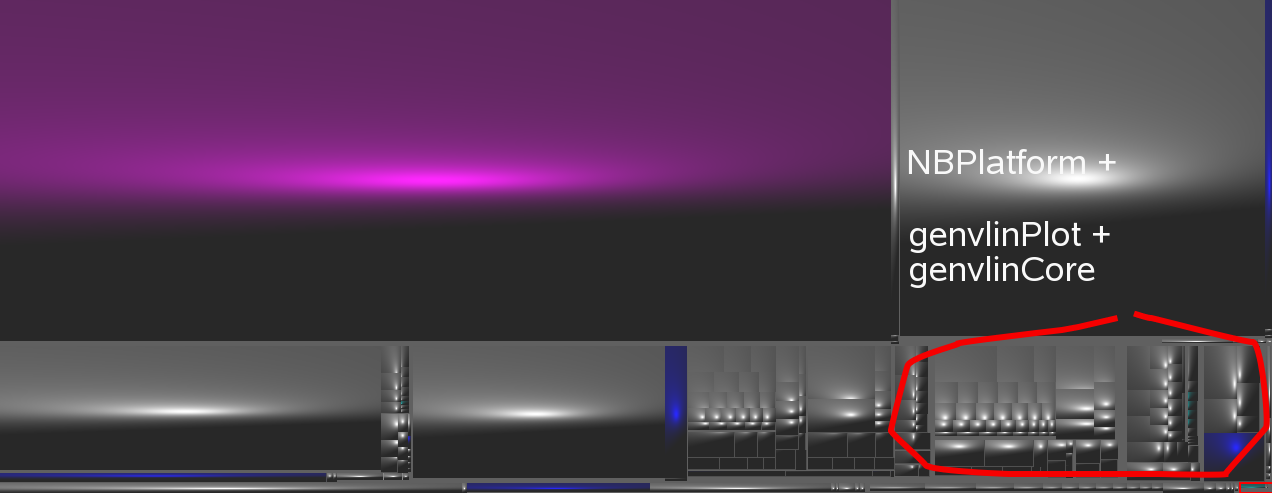
\includegraphics[width=\textwidth]{WhyIsGenvlinSoBig.png}
Only the marked area is "from genvlin" the other blocks are the used libraries:\\
JSci, JFreeChart, Beanshell, NumberCruncher, GregDennis.\\
You see: genvlin has much more potential! We should implement all the features, which are offered from all the libraries. But this requires more, developers more, time more ... :-) 
\section{Installation}
Download genvlin-nb-[version].zip from berlios. See section \ref{contact}. genvlin is written in java so you need at least the {\bf j}ava {\bf r}untime {\bf e}nvironment 1.4.2 (jre1.4.2\_?). Install the jre!\\
Then extract the zip in you home directory. E.g. /home/peter/ After extraction you will get\\ /home/peter/genvlin-nb-[version]\\ Go to /home/peter/genvlin-nb-[version]/bin and run genvlin (linux, mac) or genvlin.exe (windows).
\section{Usage}
\subsection{First Run}
If you run genvlin for the first time a "genvlin folder" is created (e.g. linux: /home/peter/.genvlin)!
All important settings of the GUI etc. are stored in this folder.\\
\subsection{Create A Table}
Go to the menuitem "window" select "favorites", if not already open. Right click a folder of your choice and choose
"New" and "All Templates". Then double click "other" and choose "Empty File" then type "test.dat" and click "Next".
You will see the import dialog. Press "Do Import". Now you see two columns called {\bf vectors} in genvlin (with no title).
\subsection{Import A Table}
Double click a file (.txt or .dat) in the favorite window. Select the column separator in the import file dialog. Then click "Do Import". Now you see two vectors in a table (with no title).
\subsection{Work With The Table}
\subsubsection{Set The Vectors Title}
Richt click the head of a vector. Type in the title and press [Enter].
\subsubsection{Select A Vector}
Click on the header. Or select a any row of the table (or only parts) and then click the header $\rightarrow$ all involved vectors will be selected.
\subsubsection{Plot Vectors}
\label{plot}
Select at least two vectors. Right click the selection. Choose "JSci"$\rightarrow$"JLineGraph" or\\ "JFreeChart"$\rightarrow$"XYLineChart" or \\ "Genvlin Plotter"$\rightarrow$"Line Plot".\\
The {\bf first} vector will be the x and any other will be the dependend y.\\
And how to change the xy-assignments?\\ Simply sort the vectors (press on the header and drag anywhere) in the manner you want!
\subsubsection{Copy And Paste In The Table}
\begin{itemize}
\item With [Control]+C you can copy some values (change the order and press again $\rightarrow$ different clipboard contents).
\item Paste with [Control]+V in your favourite text editor. 
\item Paste (overwrite) with [Control]+[Shift]+V (no undo implemented!)
\item Paste area with [Control]+[Alt]+V - where paste area means: you have to select the area and so only this area can be overwritten from the cliboard contents. And this enables you to make undo!\\
\item Cut values with [Control]+X
\item Undo with [Control]+Z (undo from paste overwrite is not imlemented!)
\end{itemize}

\subsubsection{Export}
You simply have to close the table and answer "Yes" in the dialog. Then the table will be written to the disc.
\subsection{Working With Genvlin Plotter}
Drag the mouse to measure a distance between two points.\\
Drag the mouse while holding [Shift] to zoom the plot. Right click enables you to choose a xydata, which you want to autoscale or remove!\\
Drag the mouse while holding [Control] to translate the plot.\\
{\bf Try it out!}
\subsection{Working With JFreeChart}
There are many things we can implement: various xy-plot styles and piecharts ...\\
Actually you can plot a XYLineChart. See section \ref{plot}. Then right click the panel and see whats possible:\\
Printing or saving the panel and changing various plot settings via the popupmenu.\\
Drag the mouse from the upper left corner to the bottom $\rightarrow$ zoom the plot. Dragging in any other direction will autoscale the plot again!\\
\section{License}
The most things are under the {\bf LGPL} (GNU Lesser General Public License):\\
The core of genvlin, the plotlibraries (JFreeChart+JCommon, JSci) and the Beanshell script language.\\
The netbeans platform stands under the {\bf SPL} (Sun Public License).\\
\section{Help Wanted}
Help is wanted! See the Developer Zone on the homepage! We need:\\
\begin{itemize}
\item java developer
\item web layouter
\item private or industrial sponsors
\item native english speakers to review all the doc and source
\item translators to translate the program and the doc into various languages
\item tester (with and without java knowledge)
\end{itemize}
A developer will be registered (he/she gets svn-write access) if he/she solves two small tasks or one big in the todo-list! (It is also okay if he/she send me his/her own tasks for genvlin and solved that...)
%If there are at least 10 developers I will choose the {\bf "programmer of the year"} and he/she will 
%recieved 50 EUR on his web.de account (registration is free! sorry to paypal users.)
\section{Contact}
\label{contact}
Visit the genvlin web page at: http://genvlin.berlios.de/\\
My email adress: sourcemaker2000-genvlin at yahoo dot de\\
\end{document}
